% =====================================================================
%  PHLOP -- bundled paper additions (Methodology + Results)
%  ---------------------------------------------------------------------
%  Single \input file covering the post-submission contribution:
%    * out-of-distribution (disjoint) train/val/test split
%    * per-question difficulty labels
%    * LoRA fine-tuning difficulty-curriculum ablation (2 prompt settings)
%    * fine-tuned model set: SmolVLM, Qwen2-VL, InternVL3
%    * results table + figures + defensive framing/limitations
%
%  Requirements:
%    \usepackage{booktabs}
%    \usepackage{multirow}
%    \graphicspath{{figures/}}   % copy notebooks/comparison_output/figures/* here
%
%  Defensive tweaks applied (per review): contribution reframed around
%  curriculum dependency + text-hint reliance; OOD split explicitly defended;
%  the "shortcut/cheating" claim is hedged; limitations preempt obvious
%  critiques (single run, small model set, LoRA-only).
% =====================================================================


% ---------------------------------------------------------------------
% (A) REFRAMING SNIPPETS  -- drop into the Abstract / Introduction.
% ---------------------------------------------------------------------
% Abstract, replacement sentence for the experiments line:
%
%   Beyond zero-shot evaluation, we LoRA-fine-tune three open VLMs on
%   difficulty-graded curricula under an out-of-distribution split, and find
%   that physical-reasoning accuracy is strongly curriculum-dependent and that
%   models lean heavily on textual physics hints---revealing both how these
%   models acquire physical knowledge and where they exploit non-visual
%   shortcuts.
%
% Introduction, additional contribution bullet:
%
%   \item \textbf{Learning and shortcut analysis:} Using an out-of-distribution
%   split and a difficulty-curriculum fine-tuning study, we characterize
%   \emph{how} VLMs acquire physical reasoning (curriculum dependency) and
%   \emph{where} they rely on textual shortcuts rather than visual dynamics.
% ---------------------------------------------------------------------


% =====================================================================
\subsection{Dataset Splits for Domain Generalization}
% (Section III-A, after "Parameter Sampling".)
% =====================================================================

To evaluate \emph{generalization} rather than memorization, PHLOP is partitioned
into \textsc{train}, \textsc{val}, and \textsc{test} splits whose generative
factors are deliberately \emph{disjoint}. Instead of randomly partitioning a
single pool of scenes---which would let a model exploit shared textures,
materials, or viewpoints---each split draws from a different region of the scene
parameter space: distinct object shapes, materials, per-material physical
sub-components (e.g.\ different metal alloys), object-count ranges, collision
modes, floor textures, and camera profiles. This design controls for rote
memorization and isolates compositional, out-of-distribution (OOD)
generalization: the \textsc{test} split contains material--shape--viewpoint
combinations never seen in training (e.g.\ \texttt{rubber} and \texttt{block}
objects under an ``extreme'' camera profile). Table~\ref{tab:splits} summarizes
the configuration; the full specification is released in
\texttt{split\_config.py}.

\begin{table}[t]
\centering
\caption{Disjoint generative factors per split, enforcing out-of-distribution
evaluation. Material sub-components (e.g.\ metal alloys) are also disjoint across
splits, so even shared material categories use different physical-parameter
regions.}
\label{tab:splits}
\small
\begin{tabular}{llll}
\toprule
Factor & Train & Val & Test \\
\midrule
Shapes        & ball, cube, cyl.     & ball, cube         & block, cyl., cube \\
Materials     & metal, wood, plastic & metal, wood, glass & glass, rubber \\
\#Objects     & 2--6                 & 2--5               & 3--7 \\
Camera        & broad                & narrow             & extreme \\
Collisions    & coll./slide/stat.    & coll./slide        & coll./offset/slide \\
Floor         & checker/flat         & flat/gradient      & checker/gradient \\
\bottomrule
\end{tabular}
\end{table}

Every scene is additionally rendered under two \textbf{camera modes}---a
\texttt{static} fixed-viewpoint render and a \texttt{moving} (orbiting) render.
All experiments reported here use the \texttt{static} mode.


% =====================================================================
\subsection{Question Difficulty Annotation}
% (Section III-B, after "Automatic Question Generation".)
% =====================================================================

Each generated question is tagged with a \textbf{difficulty} label---
\textit{easy}, \textit{medium}, \textit{hard}, or \textit{very\_hard}---reflecting
the depth of reasoning required rather than surface form:

\begin{itemize}
  \item \textbf{Easy}: single-step perception and counting (object count, rolling
        detection, stopped-object count, collision presence).
  \item \textbf{Medium}: property comparison and attribute inference
        (e.g.\ highest-friction object, velocity/friction scaling).
  \item \textbf{Hard} / \textbf{very\_hard}: multi-step reasoning over continuous
        dynamics (momentum/energy conservation, multi-hop causation,
        temporal-event ordering).
\end{itemize}

These labels define the fine-tuning curriculum in Section~\ref{sec:finetune}.


% =====================================================================
\subsection{Fine-tuning Protocol and Difficulty Ablation}
\label{sec:finetune}
% (Replaces / extends Section III-B-3 "Evaluation Protocol".)
% =====================================================================

Whereas our initial evaluation was restricted to zero-shot inference, we now
\textbf{LoRA-fine-tune} three open vision--language models---\textbf{SmolVLM},
\textbf{Qwen2-VL}, and \textbf{InternVL3}---and study how the \emph{difficulty
composition} of the training data affects physical reasoning. We define four
training curricula (Table~\ref{tab:ftconfig}). To measure generalization
\emph{across difficulty}, each model is validated on the difficulties
\emph{held out} of its training set; the \textit{full} curriculum trains on all
difficulties with no holdout. PHLOP thus tests generalization on two
complementary axes: \emph{domain} (unseen materials, shapes, and viewpoints,
Table~\ref{tab:splits}) and \emph{difficulty} (Table~\ref{tab:ftconfig}).

\begin{table}[t]
\centering
\caption{Fine-tuning curricula over question difficulty. Validation uses the
difficulties excluded from training (\texttt{FINE\_TUNE\_CONFIGS}).}
\label{tab:ftconfig}
\small
\begin{tabular}{lll}
\toprule
Curriculum & Train difficulties & Validation difficulties \\
\midrule
\textit{easy}         & easy         & medium, hard, very\_hard \\
\textit{easy\_medium} & easy, medium & hard, very\_hard \\
\textit{hard}         & hard         & easy, medium, very\_hard \\
\textit{full}         & all          & --- (no holdout) \\
\bottomrule
\end{tabular}
\end{table}

Each curriculum is run under two prompting settings: \textbf{no physics hint}
(video + question only) and \textbf{with physics hint} (object physical
parameters appended to the prompt). Together with the non-fine-tuned
\emph{zero-shot} baseline, this yields five conditions per model and prompting
setting, evaluated on the same held-out \textsc{test} split
($25{,}436$ questions; $22{,}635$ excluding the degenerate \textit{unknown}
bucket).


% =====================================================================
\subsection{Fine-tuning Results}
\label{sec:finetune-results}
% (New subsection in Section IV.)
% =====================================================================

\begin{table*}[t]
\centering
\caption{Answer accuracy (\%) of fine-tuned VLMs on the out-of-distribution
PHLOP test split, across the difficulty curriculum and two prompting settings.
\textit{Zero-shot} is the non-fine-tuned base model. Best per row in
\textbf{bold}.}
\label{tab:finetune-ablation}
\begin{tabular}{llccccc}
\toprule
Setting & Model & Zero-shot & Easy & Easy+Med & Hard & Full \\
\midrule
\multirow{3}{*}{No physics hint}
 & SmolVLM   & 32.9 & 65.7 & 72.7 & 60.5 & \textbf{84.4} \\
 & Qwen2-VL  & 22.6 & 20.0 & 46.0 & 37.3 & \textbf{51.6} \\
 & InternVL3 & 24.0 & 65.6 & \textbf{86.0} & 84.4 & 84.2 \\
\midrule
\multirow{3}{*}{With physics hint}
 & SmolVLM   & 32.9 & 70.4 & 80.0 & 59.1 & \textbf{88.3} \\
 & Qwen2-VL  & 17.8 & 44.8 & \textbf{68.2} & 50.7 & 64.0 \\
 & InternVL3 & 22.7 & 68.3 & \textbf{92.0} & 88.5 & 91.2 \\
\bottomrule
\end{tabular}
\end{table*}

\begin{figure*}[t]
  \centering
  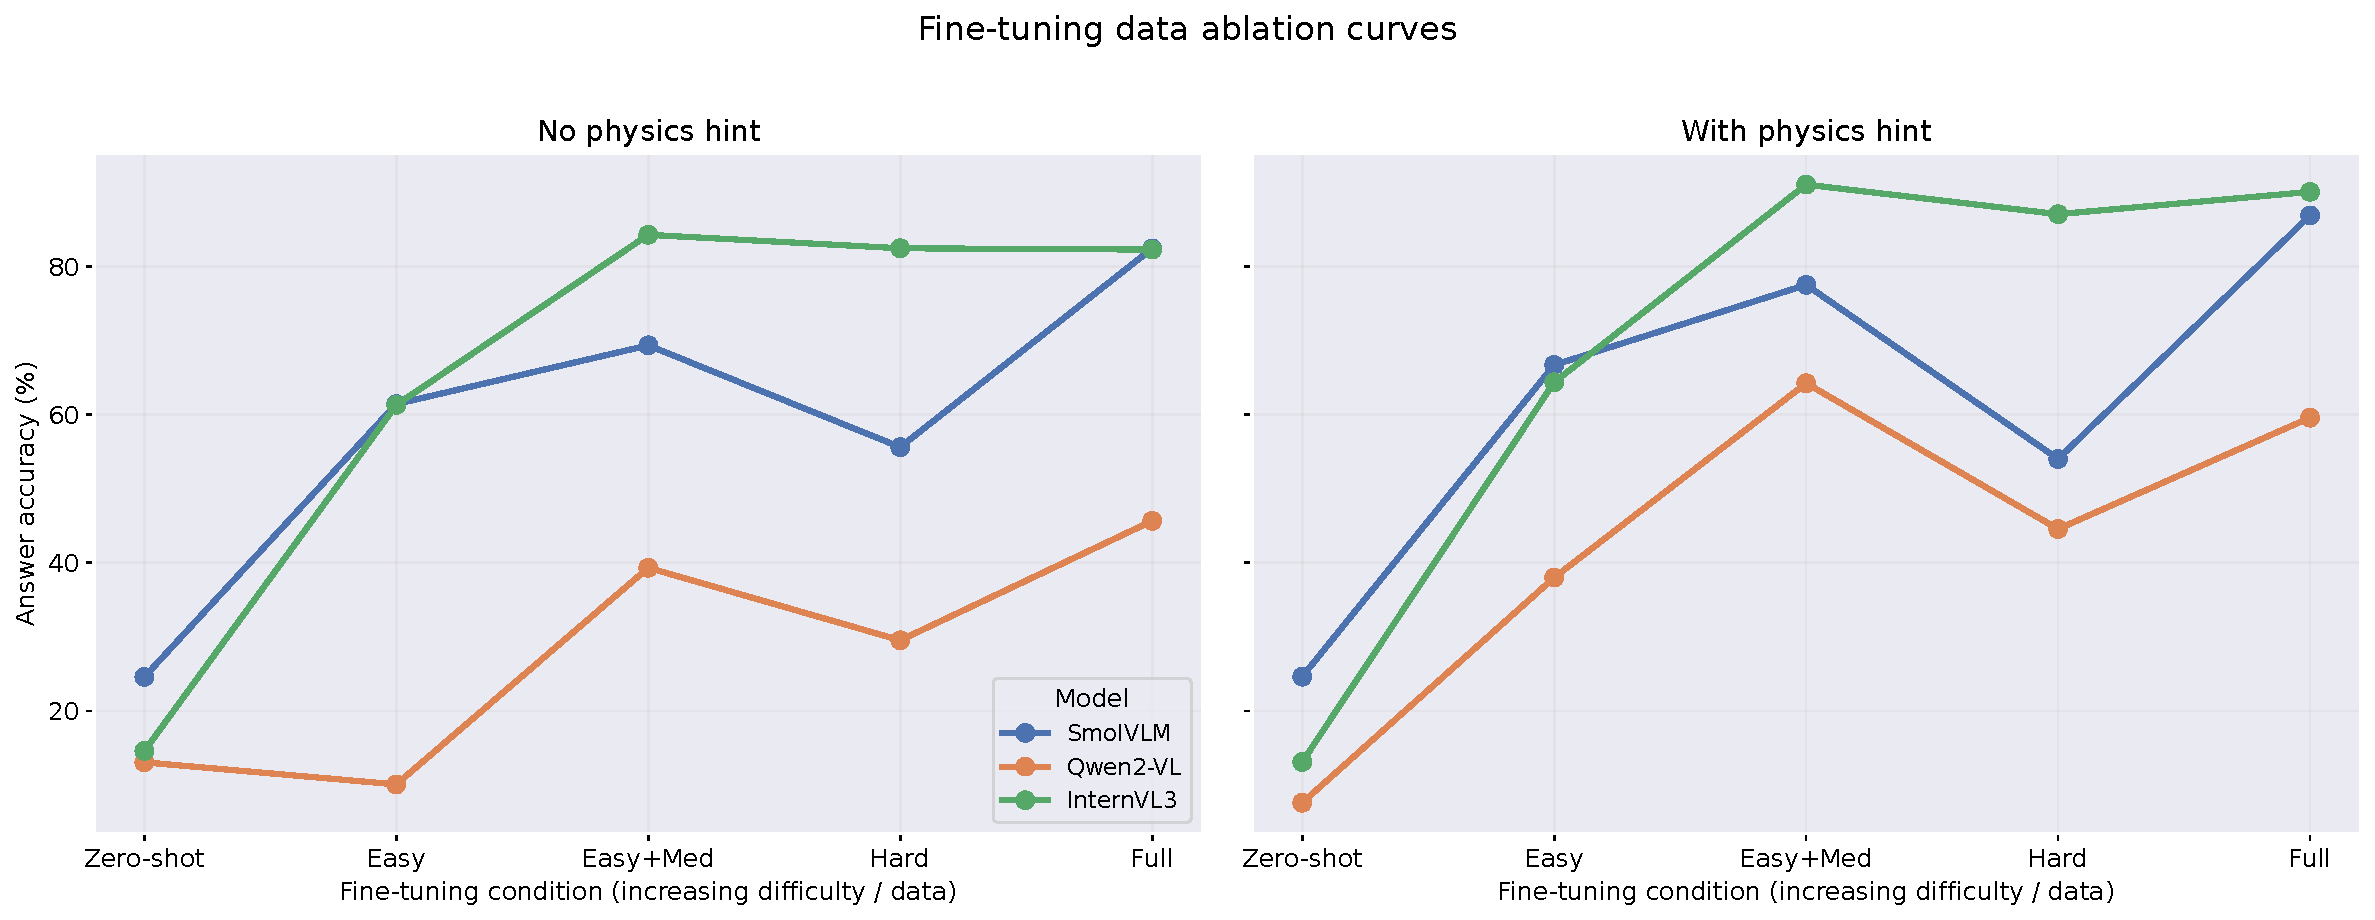
\includegraphics[width=\textwidth]{ablation_curves.pdf}
  \caption{Fine-tuning difficulty ablation. Answer accuracy vs.\ training
  curriculum for each model, under no-physics (left) and physics-hint (right)
  prompting.}
  \label{fig:ablation-curves}
\end{figure*}

\begin{figure}[t]
  \centering
  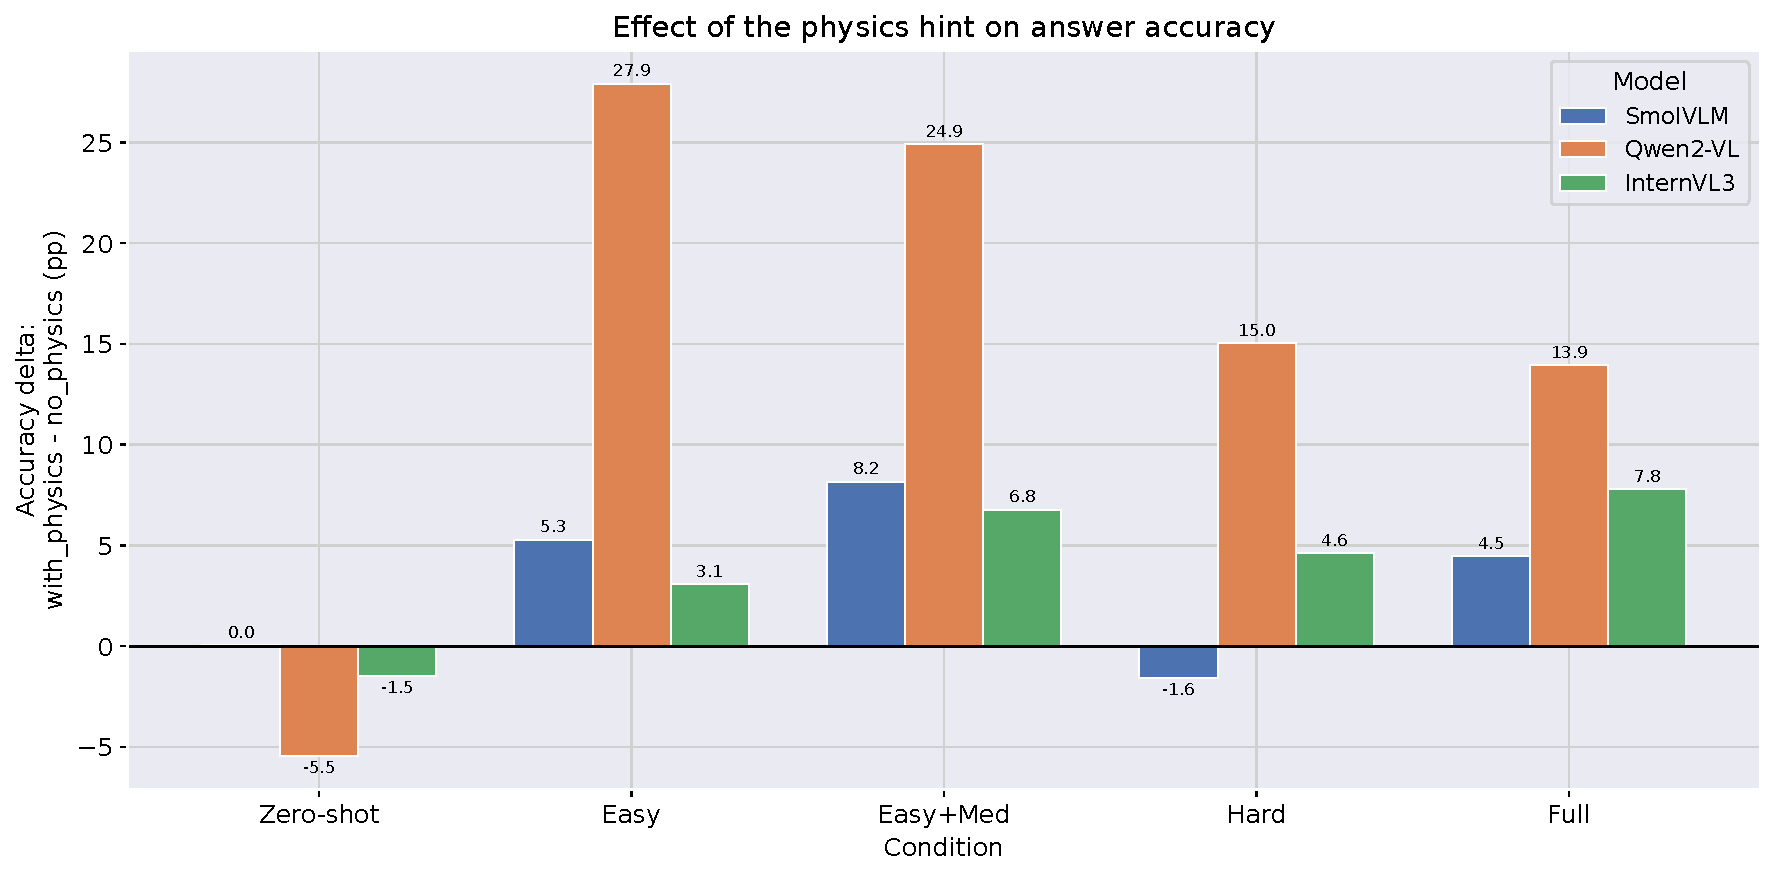
\includegraphics[width=\columnwidth]{physics_hint_delta.pdf}
  \caption{Effect of the physics hint (accuracy with hint minus without, in
  percentage points). Gains are largest for Qwen2-VL, consistent with greater
  reliance on textual cues.}
  \label{fig:physics-delta}
\end{figure}

Table~\ref{tab:finetune-ablation} and Fig.~\ref{fig:ablation-curves} reveal two
findings about \emph{how} VLMs acquire physical reasoning on PHLOP.

\textbf{Curriculum dependency.} Fine-tuning yields large gains over zero-shot for
all models (e.g.\ InternVL3: $22.7\to92.0\%$ with physics, \textit{easy\_medium}),
but these gains are \emph{not} monotonic in difficulty. For every model and
prompting setting, the \textit{hard}-only curriculum underperforms
\textit{easy\_medium} (e.g.\ SmolVLM $80.0\to59.1\%$ with physics), and accuracy
largely saturates once easy/medium data is included. This indicates that
exposure to easier examples is necessary for stable learning of harder physical
reasoning, rather than the reverse.

\textbf{Reliance on textual hints.} Adding object physical parameters to the
prompt improves accuracy for nearly all conditions, but the magnitude varies
sharply by model (Fig.~\ref{fig:physics-delta}): Qwen2-VL gains up to
$+24.8$~pp, whereas SmolVLM and InternVL3 gain only a few points. The
disproportionate benefit for the weakest visual learner is consistent with
models exploiting textual shortcuts in place of grounded visual dynamics. We
note this is suggestive rather than conclusive---physics hints can also
legitimately aid grounding---but the pattern (largest gains where visual
accuracy is lowest, e.g.\ Qwen2-VL's \textit{easy} curriculum rising
$20.0\to44.8\%$) points toward shortcut reliance. InternVL3 attains the best
overall accuracy, consistent with its stronger base architecture.


% =====================================================================
% (B) LIMITATIONS ADDITION  -- append to Section V.
% =====================================================================
% The fine-tuning study uses parameter-efficient (LoRA) adaptation rather than
% full fine-tuning, a single training run per configuration (so we report point
% estimates without seed variance), and a small set of three open models
% constrained by available hardware. The physics-hint analysis is observational;
% disentangling legitimate grounding from textual shortcutting would require
% controlled hint-ablation or counterfactual probes, which we leave to future
% work.
